\documentclass{beamer}
\usepackage{graphicx}
\usepackage{multirow}
\usepackage[utf8]{inputenc}
\usepackage[UKenglish]{babel}
\usepackage[UKenglish]{isodate}
\usepackage[style=authoryear]{biblatex}
\usepackage{tikz}
\usepackage[clock]{ifsym}
\usepackage{adjustbox}
\usepackage{booktabs}
\usepackage{csquotes}
\usepackage{array}
\usepackage[group-separator={,}]{siunitx}
\usetikzlibrary{positioning, shapes.arrows}

\usetheme{CambridgeUS}
\usecolortheme{rose}
\beamertemplatenavigationsymbolsempty
\addbibresource{../dissertation/references.bib}
\author[Paulius Dilkas]{Paulius Dilkas\\ {\small Supervisors: Dr Patrick Prosser and Dr Ciaran McCreesh}}
\title{Maximum Common Subgraph}
\subtitle{Algorithms and Algorithm Portfolios}
% TODO: change the date
\institute[]{School of Computing Science\\University of Glasgow}
\DeclareMathOperator{\E}{E}
\DeclareMathOperator{\nablaop}{\nabla}

\begin{document}

\maketitle

\begin{frame}{Outline}
  \tableofcontents
\end{frame}

\AtBeginSection[]
  {
     \begin{frame}<beamer>
     \frametitle{Outline}
     \tableofcontents[currentsection]
     \end{frame}
  }

\section{The Problem}

\begin{frame}{Maximum Common Subgraph}
  \begin{definition}
    A \emph{maximum common (induced) subgraph} between graphs $G_1$ and
    $G_2$ is a graph $G_3 = (V_3, E_3)$ such that $G_3$ is isomorphic to induced
    subgraphs of both $G_1$ and $G_2$ with $|V_3|$ maximised.
  \end{definition}
  \pause
  \begin{adjustbox}{max totalsize={0.5\textwidth}{0.5\textheight},center}
    \begin{tikzpicture}
      \begin{scope}[every node/.style={circle,draw}]
        \node (u1) [fill=gray,] at (0, 5) {$u_1$};
        \node (u2) at (0, 3) {$u_2$};
        \node (u3) at (0, 1) {$u_3$};
        \onslide<2>{\node (u4) at (2, 4) {$u_4$};}
        \onslide<2>{\node (u5) at (2, 2) {$u_5$};}
      \end{scope}
      \node (name1) at (1, 0) {$G_1$};
      \path (u1) [color=blue,ultra thick] edge node {} (u2);
      \onslide<2>{\path (u1) edge node {} (u4);}
      \onslide<2>{\path (u1) edge node {} (u5);}
      \onslide<2>{\path (u2) edge node {} (u4);}
      \onslide<2>{\path (u3) edge node {} (u4);}
      \onslide<2>{\path (u3) edge node {} (u5);}
      \begin{scope}[every node/.style={circle, draw},xshift=4cm]
        \node (v1) at (0, 5) {$v_1$};
        \onslide<2>{\node (v2) at (0, 3) {$v_2$};}
        \node (v3) at (0, 1) {$v_3$};
        \node (v4) [fill=gray] at (2, 4) {$v_4$};
        \onslide<2>{\node (v5) [fill=gray] at (2, 2) {$v_5$};}
      \end{scope}
      \node (name2) [xshift=4cm] at (1, 0) {$G_2$};
      \begin{scope}[color=blue,ultra thick]
        \onslide<2>{\path (v1) edge node {} (v2);}
        \path (v1) edge node {} (v4);
        \onslide<2>{\path (v2) edge node {} (v4);}
        \onslide<2>{\path (v2) edge node {} (v5);}
      \end{scope}
      \begin{scope}[color=red,thick]
        \onslide<3->{\path[->] (u1) edge [bend left=40] (v4);}
        \onslide<3->{\path[->] (u2) edge (v1);}
        \onslide<3->{\path[->] (u3) edge (v3);}
      \end{scope}
    \end{tikzpicture}
  \end{adjustbox}
\end{frame}

\begin{frame}{Related: Subgraph Isomorphism}
  \begin{itemize}
    \item A decision problem: is $G_1$ isomorphic to a subgraph of $G_2$?
    \item $G_1$ is the \alert{pattern} graph
    \item $G_2$ is the \alert{target} graph
  \end{itemize}
  \begin{adjustbox}{max totalsize={0.6\textwidth}{0.6\textheight},center}
    \begin{tikzpicture}
      \begin{scope}[every node/.style={circle,draw}]
        \node (u1) [fill=gray,] at (0, 5) {$u_1$};
        \node (u2) at (0, 3) {$u_2$};
        \node (u3) at (0, 1) {$u_3$};
      \end{scope}
      \node (name1) at (0, 0) {$G_1$};
      \path (u1) [color=blue,ultra thick] edge node {} (u2);
      \begin{scope}[every node/.style={circle, draw},xshift=4cm]
        \node (v1) at (0, 5) {$v_1$};
        \node (v2) at (0, 3) {$v_2$};
        \node (v3) at (0, 1) {$v_3$};
        \node (v4) [fill=gray] at (2, 4) {$v_4$};
        \node (v5) [fill=gray] at (2, 2) {$v_5$};
      \end{scope}
      \node (name2) [xshift=4cm] at (1, 0) {$G_2$};
      \begin{scope}[color=blue,ultra thick]
        \path (v1) edge node {} (v2);
        \path (v1) edge node {} (v4);
        \path (v2) edge node {} (v4);
        \path (v2) edge node {} (v5);
      \end{scope}
      \begin{scope}[color=red,thick]
        \onslide<2->{\path[->] (u1) edge [bend left=40] (v4);}
        \onslide<2->{\path[->] (u2) edge (v1);}
        \onslide<2->{\path[->] (u3) edge (v3);}
      \end{scope}
    \end{tikzpicture}
  \end{adjustbox}
\end{frame}

\begin{frame}{Why Is It Important?}
  \begin{columns}[t]
    \begin{column}{0.5\textwidth}
      \centering
      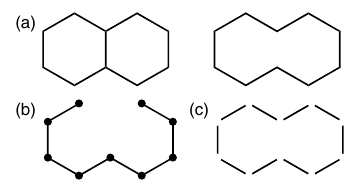
\includegraphics[width=0.9\textwidth,height=0.4\textheight,keepaspectratio]{chemistry.png} \\[-7pt]
      {\tiny Source: \cite{WCMS:WCMS5}}
      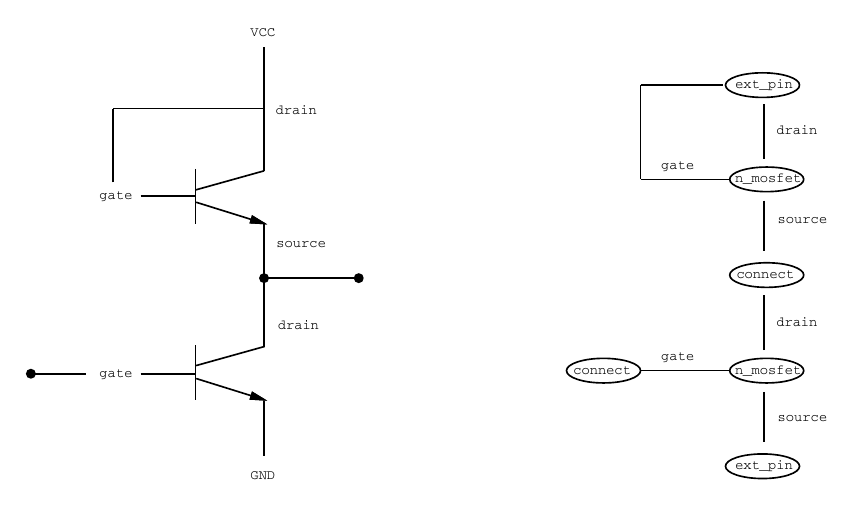
\includegraphics[width=0.9\textwidth,height=0.4\textheight,keepaspectratio]{electronics.png} \\[-7pt]
      {\tiny Source: \cite{DBLP:journals/jair/CookH94}}
    \end{column}
    \begin{column}{0.5\textwidth}
      \centering
      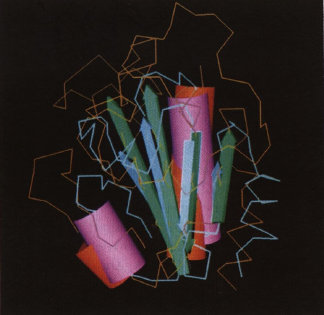
\includegraphics[width=0.9\textwidth,height=0.4\textheight,keepaspectratio]{proteins.png} \\[-7pt]
      {\tiny Source: \cite{grindley}}
      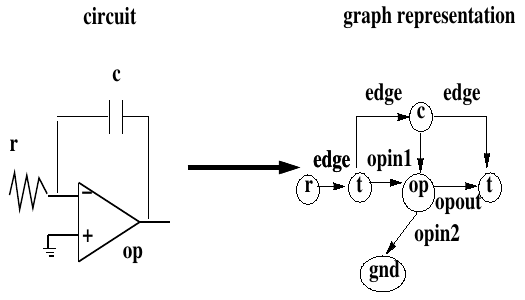
\includegraphics[width=0.9\textwidth,height=0.4\textheight,keepaspectratio]{electronics2.png} \\[-7pt]
      {\tiny Source: \cite{617051}}
    \end{column}
  \end{columns}
\end{frame}

\section{Algorithms}

\begin{frame}{Algorithms}
  \begin{itemize}
  \item \textsc{McSplit}, $\textsc{McSplit}{\downarrow}$
    \begin{itemize}
    \item \cite{DBLP:conf/ijcai/McCreeshPT17}
    \end{itemize}
  \item clique encoding
    \begin{itemize}
    \item \cite{DBLP:conf/cp/McCreeshNPS16}
    \end{itemize}
  \item $k{\downarrow}$
    \begin{itemize}
    \item \cite{DBLP:conf/aaai/HoffmannMR17}
    \end{itemize}
  \end{itemize}
\end{frame}

\begin{frame}{\textsc{McSplit}: a Branch and Bound Algorithm}
  \begin{columns}
    \begin{column}{0.5\textwidth}
      \begin{adjustbox}{max totalsize={0.9\textwidth}{0.9\textheight},center}
        \begin{tikzpicture}
          \begin{scope}[every node/.style={circle,draw}]
            \node (u1) [fill=gray,] at (0, 5) {$u_1$};
            \node (u2) at (0, 3) {$u_2$};
            \node (u3) at (0, 1) {$u_3$};
            \node (u4) at (2, 4) {$u_4$};
            \node (u5) at (2, 2) {$u_5$};
          \end{scope}
          \node (name1) at (1, 0) {$G_1$};
          \path (u1) [color=blue,ultra thick] edge node {} (u2);
          \path (u1) edge node {} (u4);
          \path (u1) edge node {} (u5);
          \path (u2) edge node {} (u4);
          \path (u3) edge node {} (u4);
          \path (u3) edge node {} (u5);
          \begin{scope}[every node/.style={circle, draw},xshift=4cm]
            \node (v1) at (0, 5) {$v_1$};
            \node (v2) at (0, 3) {$v_2$};
            \node (v3) at (0, 1) {$v_3$};
            \node (v4) [fill=gray] at (2, 4) {$v_4$};
            \node (v5) [fill=gray] at (2, 2) {$v_5$};
          \end{scope}
          \node (name2) [xshift=4cm] at (1, 0) {$G_2$};
          \begin{scope}[color=blue,ultra thick]
            \path (v1) edge node {} (v2);
            \path (v1) edge node {} (v4);
            \path (v2) edge node {} (v4);
            \path (v2) edge node {} (v5);
          \end{scope}
          \begin{scope}[color=red,thick]
            \onslide<2->{\path[->] (u1) edge [bend left=40] (v4);}
            \onslide<8->{\path[->] (u2) edge [bend right=20] (v1);}
            \onslide<5->{\path[->] (u3) edge [] (v3);}
          \end{scope}
        \end{tikzpicture}
      \end{adjustbox}
    \end{column}

    \begin{column}{0.5\textwidth}
      \begin{overprint}
        Partial solution: \only<4>{\alert{$u_1 \mapsto v_4$}}\only<5-6>{$u_1 \mapsto v_4$}\only<7>{$u_1 \mapsto v_4$, \alert{$u_3 \mapsto v_3$}}\only<8->{$u_1 \mapsto v_4$, $u_3 \mapsto v_3$}

        Upper bound: \only<1-3>{$4$}\only<4>{\alert{$1+2$}}\only<5-6>{$1+2$}\only<7>{\alert{$2+1$}}\only<8->{$2+1$}
      \end{overprint}
      \begin{table}
        \begin{overlayarea}{\textwidth}{3cm}
          \centering
          \only<-2>{
            \begin{tabular}{c c c}
              \toprule
              Label & $G_1$ & $G_2$ \\
              \midrule
              0 & $u_2, u_3, u_4, u_5$ & $v_1, v_2, v_3$ \\
              1 & $u_1$ & $v_4, v_5$ \\
              \bottomrule
            \end{tabular}
          }
          \only<3>{
            \begin{tabular}{c c c}
              \toprule
              Label & $G_1$ & $G_2$ \\
              \midrule
              00 & $u_3$ & $v_3$ \\
              01 & $u_4, u_5$ & $\emptyset$ \\
              02 & $u_2$ & $v_1, v_2$ \\
              10 & $\emptyset$ & $v_5$ \\
              \bottomrule
            \end{tabular}
          }
          \only<4-5>{
            \begin{tabular}{c c c}
              \toprule
              Label & $G_1$ & $G_2$ \\
              \midrule
              00 & $u_3$ & $v_3$ \\
              01 & $u_2$ & $v_1, v_2$ \\
              \bottomrule
            \end{tabular}
          }
          \only<6>{
            \begin{tabular}{c c c}
              \toprule
              Label & $G_1$ & $G_2$ \\
              \midrule
              010 & $u_2$ & $v_1, v_2$ \\
              011 & $u_4, u_5$ & $\emptyset$ \\
              \bottomrule
            \end{tabular}
          }
          \only<7->{
            \begin{tabular}{c c c}
              \toprule
              Label & $G_1$ & $G_2$ \\
              \midrule
              010 & $u_2$ & $v_1, v_2$ \\
              \bottomrule
            \end{tabular}
          }
        \end{overlayarea}
      \end{table}
      \begin{overprint}
        \onslide<2>
        Decision: $u_1 \mapsto v_4$
        \onslide<5>
        Decision: $u_3 \mapsto v_3$
        \onslide<8>
        Decision: $u_2 \mapsto v_1$\\ Found a solution! \\ Backtrack to confirm optimality
      \end{overprint}
    \end{column}
  \end{columns}
\end{frame}

\begin{frame}{$k{\downarrow}$}
  \begin{itemize}
  \item $k = 0$: search for a complete subgraph isomorphism
  \item $k = 1$: allow one vertex of the smaller graph to not match anything
  \item ... and so on
  \item Developed to handle large instances
  \item Implements many domain filtering techniques
  \end{itemize}
\end{frame}

\begin{frame}{$\textsc{McSplit}{\downarrow}$}
  \begin{itemize}
  \item The main idea of $k{\downarrow}$ applied to \textsc{McSplit}
  \item Looks for a common subgraph of a set size
    \begin{itemize}
    \item (decreasing with every iteration)
    \end{itemize}
  \item This allows us to prune more search tree branches
  \end{itemize}
\end{frame}

\begin{frame}{Clique Encoding}
  \begin{columns}
    \begin{column}{0.3\textwidth}
      \begin{adjustbox}{max totalsize={0.9\textwidth}{0.9\textheight},center}
        \begin{tikzpicture}
          \begin{scope}[every node/.style={circle,draw}]
            \node (u1) [fill=gray,] at (0, 5) {$u_1$};
            \node (u2) at (0, 3) {$u_2$};
            \node (u3) at (0, 1) {$u_3$};
            \node (u4) at (2, 4) {$u_4$};
            \node (u5) at (2, 2) {$u_5$};
          \end{scope}
          \path (u1) [color=blue,ultra thick] edge node {} (u2);
          \path (u1) edge node {} (u4);
          \path (u1) edge node {} (u5);
          \path (u2) edge node {} (u4);
          \path (u3) edge node {} (u4);
          \path (u3) edge node {} (u5);
          \begin{scope}[every node/.style={circle, draw},xshift=4cm]
            \node (v1) at (0, 5) {$v_1$};
            \node (v2) at (0, 3) {$v_2$};
            \node (v3) at (0, 1) {$v_3$};
            \node (v4) [fill=gray] at (2, 4) {$v_4$};
            \node (v5) [fill=gray] at (2, 2) {$v_5$};
          \end{scope}
          \begin{scope}[color=blue,ultra thick]
            \path (v1) edge node {} (v2);
            \path (v1) edge node {} (v4);
            \path (v2) edge node {} (v4);
            \path (v2) edge node {} (v5);
          \end{scope}
          \begin{scope}[color=red,thick]
            \path[->] (u1) edge [bend left=40] (v4);
            \path[->] (u2) edge [bend right=20] (v1);
            \path[->] (u3) edge [] (v3);
          \end{scope}
        \end{tikzpicture}
      \end{adjustbox}
    \end{column}

    \begin{column}{0.7\textwidth}
      \begin{adjustbox}{max totalsize={0.9\textwidth}{0.9\textheight},center}
        \begin{tikzpicture}
          \begin{scope}[every node/.style={circle,draw}]
            \node (u1v4) [color=red,ultra thick,text=black] at (360/14 * 1:9cm) {$u_1 \mapsto v_4$};
            \node (u1v5) at (360/14 * 2:9cm) {$u_1 \mapsto v_5$};
            \node (u2v1) [color=red,ultra thick,text=black] at (360/14 * 3:9cm) {$u_2 \mapsto v_1$};
            \node (u2v2) at (360/14 * 4:9cm) {$u_2 \mapsto v_2$};
            \node (u2v3) at (360/14 * 5:9cm) {$u_2 \mapsto v_3$};
            \node (u3v1) at (360/14 * 6:9cm) {$u_3 \mapsto v_1$};
            \node (u3v2) at (360/14 * 7:9cm) {$u_3 \mapsto v_2$};
            \node (u3v3) [color=red,ultra thick,text=black] at (360/14 * 8:9cm) {$u_3 \mapsto v_3$};
            \node (u4v1) at (360/14 * 9:9cm) {$u_4 \mapsto v_1$};
            \node (u4v2) at (360/14 * 10:9cm) {$u_4 \mapsto v_2$};
            \node (u4v3) at (360/14 * 11:9cm) {$u_4 \mapsto v_3$};
            \node (u5v1) at (360/14 * 12:9cm) {$u_5 \mapsto v_1$};
            \node (u5v2) at (360/14 * 13:9cm) {$u_5 \mapsto v_2$};
            \node (u5v3) at (360/14 * 14:9cm) {$u_5 \mapsto v_3$};
          \end{scope}

          \begin{scope}[color=red,ultra thick]
            \path (u1v4) edge (u2v1) edge (u3v3);
            \path (u2v1) edge (u3v3);
          \end{scope}

          \path (u1v4) edge (u2v2);
          \path (u1v5) edge (u2v2) edge (u3v1) edge (u3v3);
          \path (u2v1) edge (u5v3);
          \path (u2v2) edge (u3v3) edge (u5v3);
          \path (u2v3) edge (u3v1) edge (u3v2) edge (u5v1) edge (u5v2);
          \path (u4v1) edge (u5v3);
          \path (u4v2) edge (u5v3);
          \path (u4v3) edge (u5v1) edge (u5v2);
        \end{tikzpicture}
      \end{adjustbox}
    \end{column}
  \end{columns}
\end{frame}

\section{Algorithm Selection}

\begin{frame}{(Per-Instance) Algorithm Selection}
  \begin{definition}[\cite{DBLP:journals/ai/BischlKKLMFHHLT16}]
    Given a set $\mathcal{I}$ of problem instances, a space of algorithms
    $\mathcal{A}$, and a performance measure $m \colon \mathcal{I} \times
    \mathcal{A} \to \mathbb{R}$, the \emph{algorithm selection problem} is to
    find a mapping $s \colon \mathcal{I} \to \mathcal{A}$ that optimises
    $\mathbb{E}[m(i, s(i))]$.
  \end{definition}
    \centering
    \begin{tikzpicture}
      \onslide<2->{\node (graphs) at (0, 4) {$(G_1, G_2)$};}
      \onslide<3->{\node (features) at (2, 4) {$\begin{bmatrix}f_1\\ \vdots \\ f_n\end{bmatrix}$};}
      \onslide<4->{\node[draw] (ml) at (5, 4) {ML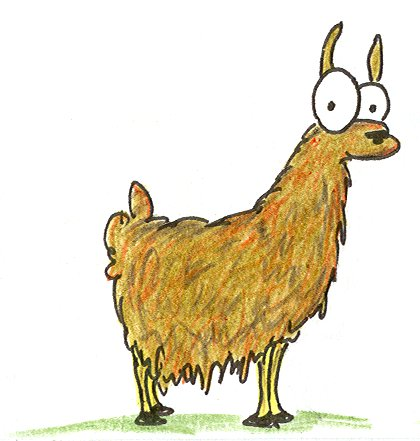
\includegraphics[scale=0.1]{llama.jpg}};}
      \onslide<5->{\node (mcsplit) at (2, 2) {\textsc{McSplit}};}
      \onslide<5->{\node (mcsplitdown) at (4, 2) {$\textsc{McSplit}{\downarrow}$};}
      \onslide<5->{\node (clique) at (6, 2) {clique};}
      \onslide<5->{\node (kdown) at (8, 2) {$k{\downarrow}$};}
      \onslide<7->{\node (answer) at (4, 0) {answer};}
      \path[->]<3-> (graphs) edge node[above] {\VarClock} (features);
      \path[->]<4-> (features) edge (ml);
      \path[->]<5-> (ml) edge (mcsplit);
      \only<1-5>{\tikzset{properties/.style={}}}
      \only<6->{\tikzset{properties/.style={ultra thick}}}
      \draw<5-> [->] (ml) edge[properties] (mcsplitdown);
      \path[->]<5-> (ml) edge (clique);
      \path[->]<5-> (ml) edge (kdown);
      \path[->]<7-> (mcsplitdown) edge node[right] {\VarClock} (answer);
      \path[->]<7-> (graphs) edge [bend right=50] (4, 1);
    \end{tikzpicture}
\end{frame}

\begin{frame}{Labelling}
  Data from \cite{foggia2001-2, DBLP:journals/prl/SantoFSV03}
  (\num{81400} pairs of graphs)
  \pause
  \begin{definition}
    A \emph{vertex-labelled graph} is a 3-tuple $G = (V, E, \mu)$, where $\mu
    \colon V \to \{ 0, \dots, N - 1 \}$ is a vertex labelling function, for some
    $N \in \mathbb{N}$.
  \end{definition}
  \pause
  \begin{definition}
    A graph $G = (V, E, \mu)$ is said to have a \emph{$p\%$ (vertex) labelling} if
    \[ N = \max \left\{ 2^n : n \in \mathbb{N},\, 2^n < \left\lfloor \frac{p}{100\%}
          \times |V| \right\rfloor \right\}. \]
  \end{definition}
\end{frame}

\begin{frame}{Labelling}
  \begin{definition}
    A graph $G = (V, E, \mu)$ is said to have a \emph{$p\%$ (vertex) labelling} if
    \[ N = \max \left\{ 2^n : n \in \mathbb{N},\, 2^n < \left\lfloor \frac{p}{100\%}
          \times |V| \right\rfloor \right\}. \]
  \end{definition}
  \begin{itemize}
  \item 5\% labelling - 20 vertices per label on average
  \item 50\% labelling - 2 vertices per label on average
    \pause
  \item Typical values explored: 33\%, 50\%, 75\%
    \pause
  \item In my data: 5\%, 10\%, 15\%, 20\%, 25\%, 33\%, 50\%
    \pause
  \item 3 different cases:
    \begin{itemize}
    \item no labels
    \item vertex labels
    \item vertex and edge labels
    \end{itemize}
  \end{itemize}
\end{frame}

\begin{frame}{Number of Vertices Per Label}
  \begin{figure}
    \centering
    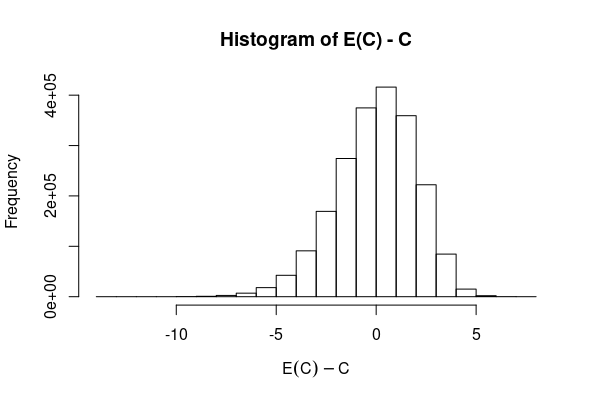
\includegraphics[scale=0.4]{../dissertation/images/labelling_histogram.png}
  \end{figure}
  For each graph and label
  \begin{itemize}
  \item $C$ is the number of vertices with that label
  \item $\E(C)$ is the number we would expect from a (discrete) uniform distribution
  \end{itemize}
\end{frame}

\begin{frame}{Features (34 in total)}
  1--8 are from \cite{DBLP:conf/lion/KotthoffMS16}
  \begin{enumerate}
  \item number of vertices
  \item number of edges
  \item mean/max degree
  \item density
  \item mean/max distance between pairs of vertices
  \item number of loops
  \item proportion of vertex pairs with distance $\ge$ 2, 3, 4
  \item connectedness
    \pause
  \item standard deviation of degrees
  \item labelling percentage
    \pause
  \item ratios of features 1--5
  \end{enumerate}
\end{frame}

\begin{frame}{Random Forests \parencite{DBLP:journals/ml/Breiman01}}
  \begin{figure}
    \centering
    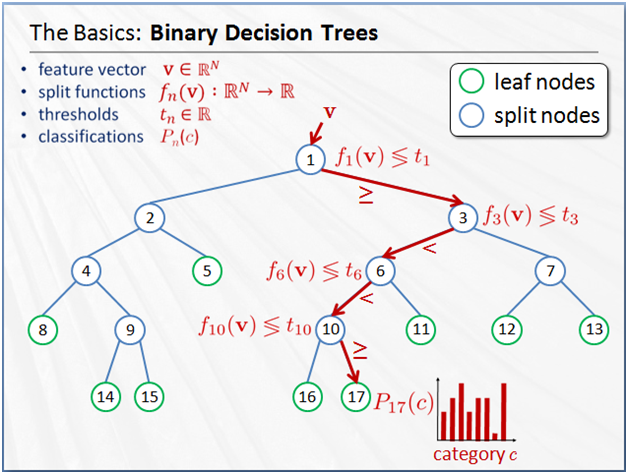
\includegraphics[scale=0.5]{random_forests_2.png} \\
    {\tiny\color{gray}Source: Tae-Kyun Kim \& Bjorn Stenger, Intelligent Systems and Networks (ISN) Research Group,\\[-7pt] Imperial College London}
  \end{figure}
\end{frame}

\begin{frame}{Random Forests \parencite{DBLP:journals/ml/Breiman01}}
  \begin{figure}
    \centering
    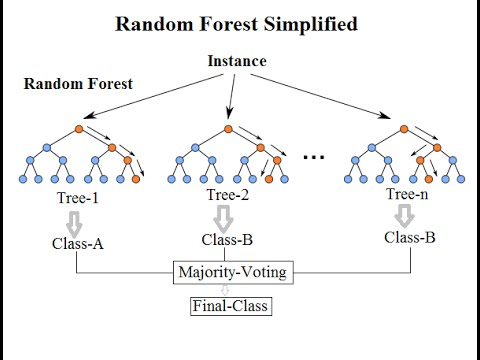
\includegraphics[scale=0.5]{rand-forest-1.jpg} \\
    {\tiny\color{gray}Source: Random Forests(r), Explained, Ilan Reinstein, KDnuggets}
  \end{figure}
\end{frame}

\begin{frame}{Results}
  \begin{figure}
    \centering
    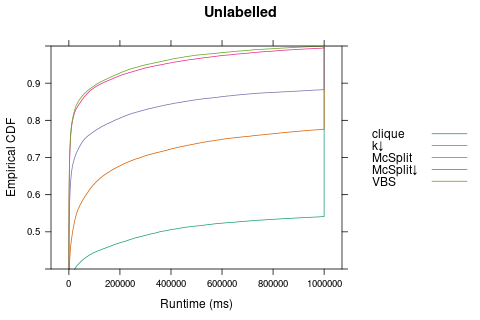
\includegraphics[width=0.9\textwidth]{../dissertation/images/ecdf_unlabelled.png}
  \end{figure}
\end{frame}

\begin{frame}{Results (27\%)}
  \begin{figure}
    \centering
    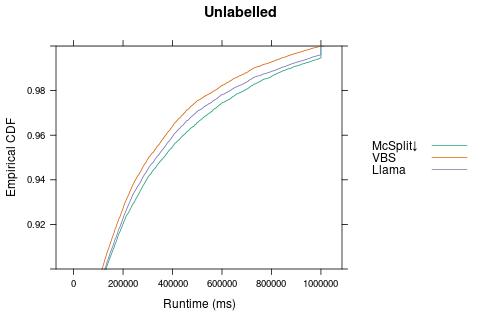
\includegraphics[width=0.9\textwidth]{../dissertation/images/ecdf_unlabelled_llama.png}
  \end{figure}
\end{frame}

\begin{frame}{Results}
  \begin{figure}
    \centering
    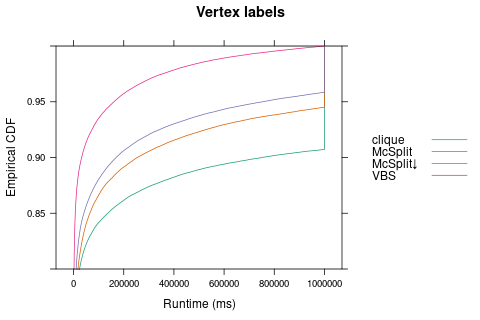
\includegraphics[width=0.9\textwidth]{../dissertation/images/ecdf_vertex_labels.png}
  \end{figure}
\end{frame}

\begin{frame}{Results (86\%)}
  \begin{figure}
    \centering
    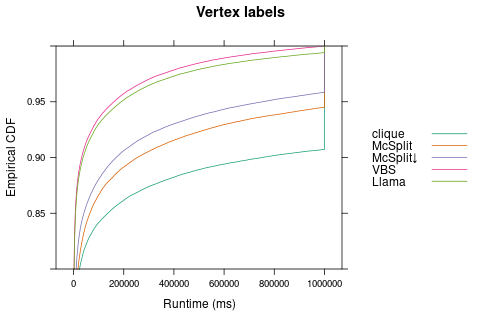
\includegraphics[width=0.9\textwidth]{../dissertation/images/ecdf_vertex_labels_llama.png}
  \end{figure}
\end{frame}

\begin{frame}{Results}
  \begin{figure}
    \centering
    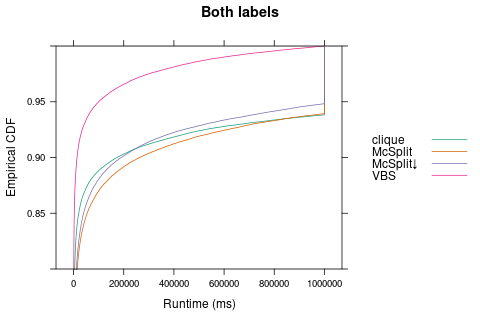
\includegraphics[width=0.9\textwidth]{../dissertation/images/ecdf_both_labels.png}
  \end{figure}
\end{frame}

\begin{frame}{Results (88\%)}
  \begin{figure}
    \centering
    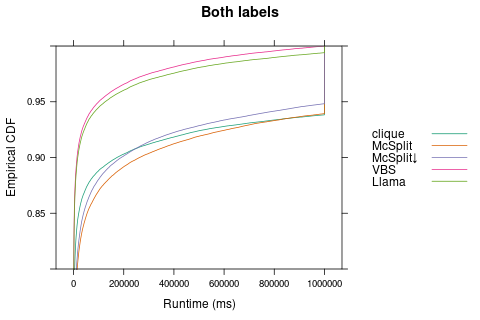
\includegraphics[width=0.9\textwidth]{../dissertation/images/ecdf_both_labels_llama.png}
  \end{figure}
\end{frame}

\begin{frame}{Errors}
  \begin{itemize}
  \item Out-of-bag error
  \item For each algorithm
    \begin{itemize}
    \item $1 - \text{recall}$
    \end{itemize}
  \end{itemize}
  \begin{definition}
    For an algorithm $A$, \emph{recall} (sensitivity) is
    \[ \frac{\text{the number of instances that were correctly predicted as
          $A$}}{\text{the number of instances where $A$ is the correct
          prediction}}. \]
  \end{definition}
\end{frame}

\begin{frame}{Errors (\%)}
  \centering
  \begin{tabular}{l c c c}
    \toprule
    \multirow{2}{*}{Error} & \multicolumn{3}{c}{Labelling} \\
    \cmidrule(lr){2-4}
                           & no & vertex & both \\
    \midrule
    out-of-bag & 17 & 13 & 14 \\
    clique & 30 & 8 & 7 \\
    \textsc{McSplit} & 29 & 22 & 29 \\
    $\textsc{McSplit}\downarrow$ & 11 & 11 & 11 \\
    $k\downarrow$ & 80 & & \\
    \bottomrule
  \end{tabular}
\end{frame}

\begin{frame}{Convergence of Errors for Unlabelled Graphs}
  \begin{figure}
    \centering
    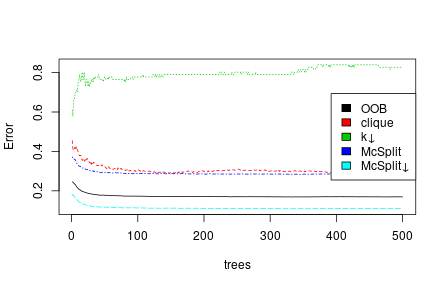
\includegraphics[scale=0.5]{../dissertation/images/unlabelled_forest_errors.png}
  \end{figure}
\end{frame}

\section{Observations and Insights}

\begin{frame}{Overview}
  \begin{itemize}
  \item Most important features:
    \begin{itemize}
    \item labelling percentage
    \item standard deviation of degrees (for both graphs)
    \end{itemize}
  \item Looking at a single feature is not enough
    \pause
  \item $k{\downarrow}$ is no longer competitive
  \item Unclear when \textsc{McSplit} outperforms $\textsc{McSplit}{\downarrow}$
    \pause
  \item Benchmarking algorithms with just a few different labels is important
  \item No work has ben done on non-uniform distributions of labels
  \end{itemize}
\end{frame}

\begin{frame}{What Happens When Labelling Changes?}
  \begin{columns}
    \begin{column}{0.5\textwidth}
      \centering
      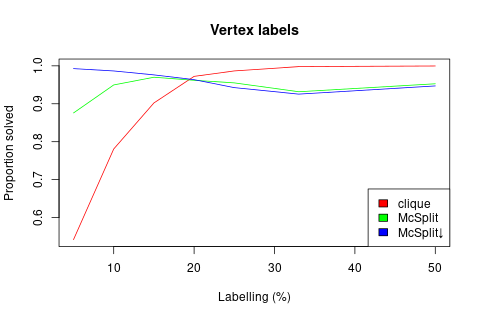
\includegraphics[width=0.9\textwidth]{../dissertation/images/vertex_labels_linechart.png}
      \visible<2>{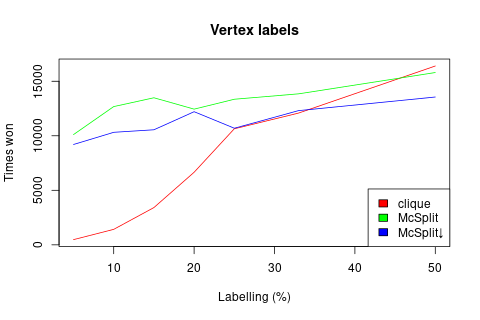
\includegraphics[width=0.9\textwidth]{../dissertation/images/vertex_labels_linechart3.png}}
    \end{column}
    \begin{column}{0.5\textwidth}
      \centering
      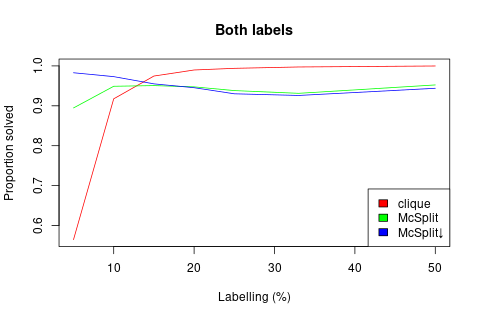
\includegraphics[width=0.9\textwidth]{../dissertation/images/both_labels_linechart.png}
      \visible<2>{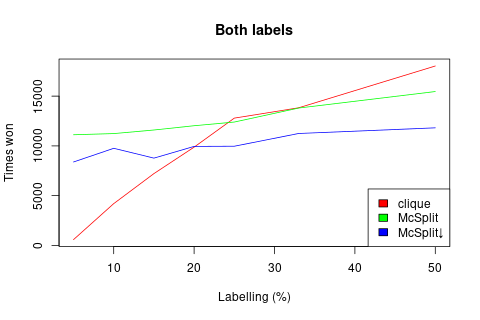
\includegraphics[width=0.9\textwidth]{../dissertation/images/both_labels_linechart3.png}}
    \end{column}
  \end{columns}
\end{frame}

\begin{frame}{Margins}
  \begin{definition}
    Let $c_1, \dots, c_n$ be $n$ \alert{classes} and let $p$ be a \alert{data point} that belongs
    to class $c_p$. Let $v_1, \dots, v_n$ denote the \alert{number of votes} for each
    class when given $p$ as input. The \alert{\emph{margin}} of $p$ is
    \[ \frac{v_p}{\sum_{i=1}^n v_i} - \max_{i \ne p} \frac{v_i}{\sum_{j=1}^n v_j}, \]
    which is a number in $[-1, 1]$.
  \end{definition}
\end{frame}

\begin{frame}{Margins: Unlabelled Graphs}
  \begin{columns}[t]
    \begin{column}{0.5\textwidth}
      \centering
      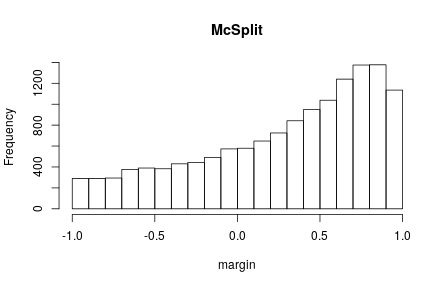
\includegraphics[width=\textwidth,height=0.4\textheight,keepaspectratio]{../dissertation/images/mcsplit_hist.png}
      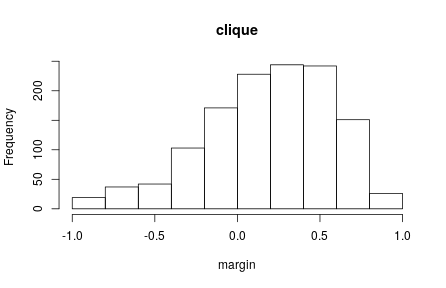
\includegraphics[width=0.9\textwidth,height=0.4\textheight,keepaspectratio]{../dissertation/images/clique_hist.png}
    \end{column}
    \begin{column}{0.5\textwidth}
      \centering
      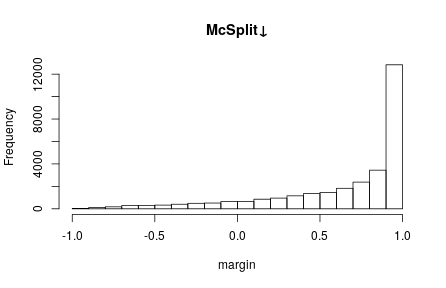
\includegraphics[width=\textwidth,height=0.4\textheight,keepaspectratio]{../dissertation/images/mcsplitdown_hist.png}
      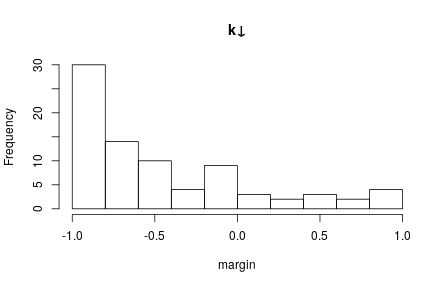
\includegraphics[width=\textwidth,height=0.4\textheight,keepaspectratio]{../dissertation/images/kdown_hist.png}
    \end{column}
  \end{columns}
\end{frame}

\begin{frame}{Margins: Vertex and Edge Labels}
  \begin{columns}[t]
    \begin{column}{0.5\textwidth}
      \centering
      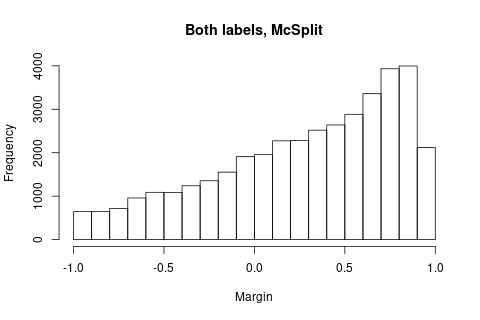
\includegraphics[width=\textwidth,height=0.4\textheight,keepaspectratio]{../dissertation/images/both_labels_mcsplit_hist.png}
      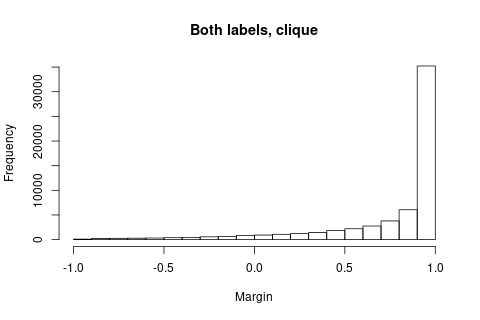
\includegraphics[width=0.9\textwidth,height=0.4\textheight,keepaspectratio]{../dissertation/images/both_labels_clique_hist.png}
    \end{column}
    \begin{column}{0.5\textwidth}
      \centering
      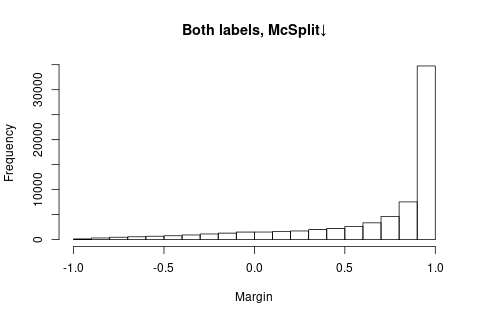
\includegraphics[width=\textwidth,height=0.4\textheight,keepaspectratio]{../dissertation/images/both_labels_mcsplitdown_hist.png}
    \end{column}
  \end{columns}
\end{frame}

\begin{frame}{Partial Dependence: Unlabelled Graphs}
  \begin{columns}
    \begin{column}{0.5\textwidth}
      \centering
      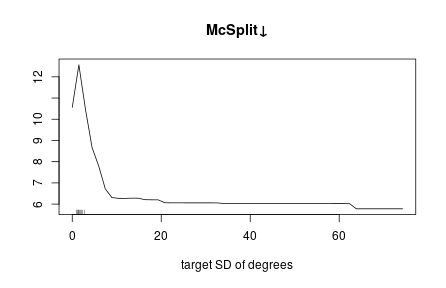
\includegraphics[width=0.8\textwidth,height=0.8\textheight,keepaspectratio]{../dissertation/images/mcsplit_partial.png}
    \end{column}
    \begin{column}{0.5\textwidth}
      \centering
      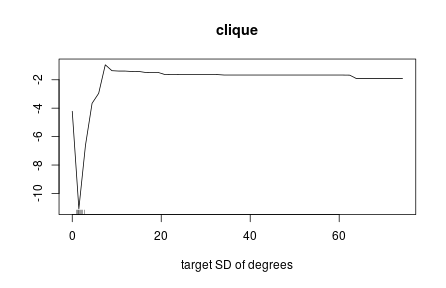
\includegraphics[width=0.8\textwidth,height=0.8\textheight,keepaspectratio]{../dissertation/images/clique_partial.png}
    \end{column}
  \end{columns}
  \begin{block}{Defined as}
    \[ f(x) = \log{p_k(x)} - \frac{1}{K} \sum_{i=1}^K \log{p_i(x)} \]
    \begin{itemize}
    \item $p_i(x)$ is the proportion of votes for class $i$
    \item $K$ is the number of different classes
    \item $k$ is the class under consideration
    \end{itemize}
  \end{block}
\end{frame}

\begin{frame}{Partial Dependence: Vertex and Edge Labels}
  \begin{columns}
    \begin{column}{0.5\textwidth}
      \centering
      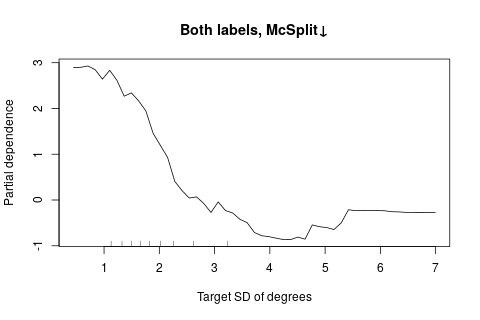
\includegraphics[width=\textwidth,height=0.4\textheight,keepaspectratio]{../dissertation/images/both_labels_mcsplitdown_stddeg.png}
      \visible<2->{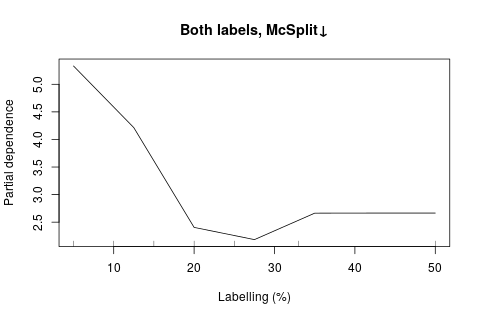
\includegraphics[width=\textwidth,height=0.4\textheight,keepaspectratio]{../dissertation/images/both_labels_mcsplitdown_labelling.png}}
    \end{column}
    \begin{column}{0.5\textwidth}
      \centering
      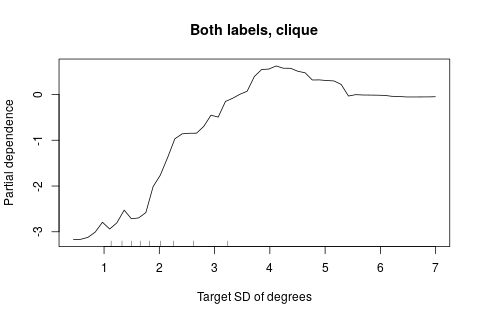
\includegraphics[width=\textwidth,height=0.4\textheight,keepaspectratio]{../dissertation/images/both_labels_clique_stddeg.png}
      \visible<2->{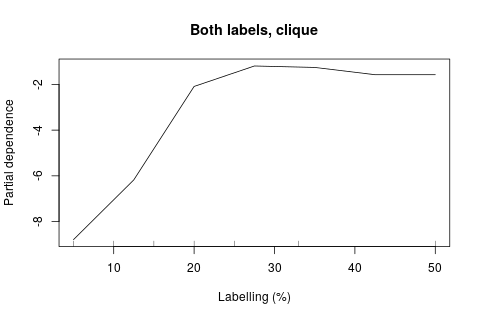
\includegraphics[width=\textwidth,height=0.4\textheight,keepaspectratio]{../dissertation/images/both_labels_clique_labelling.png}}
    \end{column}
  \end{columns}
\end{frame}

\begin{frame}{Features of the Association Graph}
  \pause
  \begin{columns}
    \begin{column}{0.5\textwidth}
      \centering
      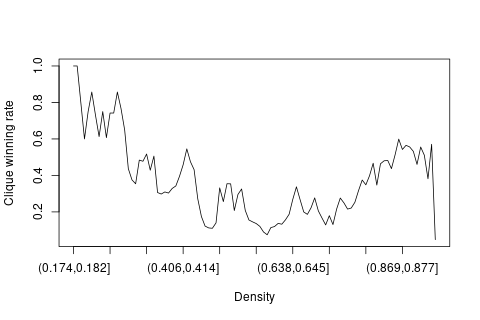
\includegraphics[width=\textwidth,height=0.4\textheight,keepaspectratio]{../dissertation/images/density_bins.png}
      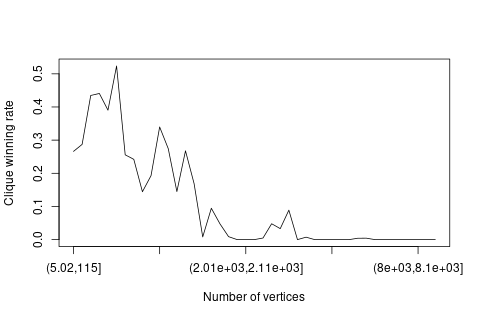
\includegraphics[width=\textwidth,height=0.4\textheight,keepaspectratio]{../dissertation/images/vertices_bins.png}
    \end{column}
    \begin{column}{0.5\textwidth}
      \centering
      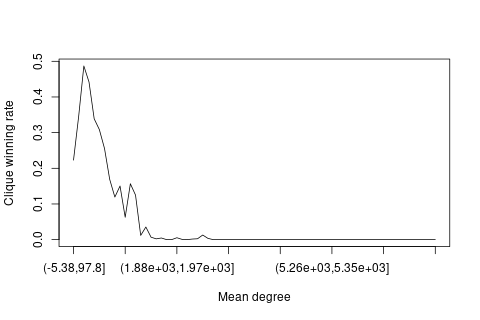
\includegraphics[width=\textwidth,height=0.4\textheight,keepaspectratio]{../dissertation/images/meandeg_bins.png}
      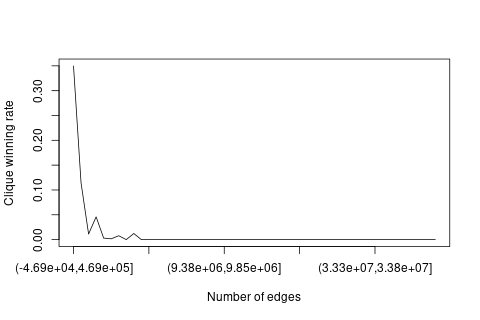
\includegraphics[width=\textwidth,height=0.4\textheight,keepaspectratio]{../dissertation/images/edges_bins.png}
    \end{column}
  \end{columns}
\end{frame}

\section{Switching Algorithms Mid-Execution}

\begin{frame}{Idea 1: Switch After a Fixed Number of Decisions}
  \pause
  \begin{itemize}
  \item Vertices of the association graph can be constructed from \textsc{McSplit}
    label classes, edges from the original input graphs
  \item Only a few extra lines of code:
    \[ |\textit{incumbent}_{\text{clique}}| \gets
      |\textit{incumbent}_{\text{\textsc{McSplit}}}| - |M| \]
    and then
    \[ \textit{incumbent}_{\textsc{McSplit}} \gets
      \textit{incumbent}_{\textsc{McSplit}} \cup
      \textit{incumbent}_{\text{clique}} \]
  \end{itemize}
\end{frame}

\begin{frame}{Not That Good...}
  \centering
  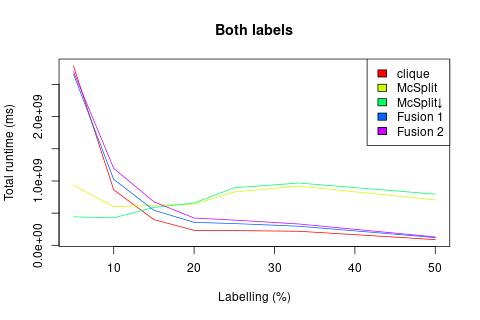
\includegraphics[scale=0.5]{../dissertation/images/fusion_linechart.png}
\end{frame}

\begin{frame}{Idea 2: From Partially Solved to Unsolved Instances}
\begin{itemize}
\item Goal: switch algorithms in a more intelligent way
\item Plan: use runtime data on unsolved instances
  \begin{itemize}
  \item using either machine learning or simple guidelines
  \end{itemize}
  \pause
\item Implementation can be optimised to:
  \begin{itemize}
  \item only track important information
  \item reuse information between iterations
  \end{itemize}
  \pause
\item Is it any good?
  \pause
  \begin{itemize}
  \item Remains to be seen
  \item Could be that...
    \pause
    \begin{itemize}
    \item the answer is ``never switch''
    \item or the performance gains are minimal
    \end{itemize}
  \end{itemize}
\end{itemize}
\end{frame}

\begin{frame}{Idea 2: From Partially Solved to Unsolved Instances}
  \begin{columns}
    \begin{column}{0.5\textwidth}
      \begin{adjustbox}{max totalsize={0.9\textwidth}{0.4\textheight},center}
        \begin{tikzpicture}
          \begin{scope}[every node/.style={circle,draw}]
            \node (u1) [fill=gray,] at (0, 5) {$u_1$};
            \node (u2) at (0, 3) {$u_2$};
            \node (u3) at (0, 1) {$u_3$};
            \node (u4) at (2, 4) {$u_4$};
            \node (u5) at (2, 2) {$u_5$};
          \end{scope}
          \node (name1) at (1, 0) {$G_1$};
          \path (u1) [color=blue,ultra thick] edge node {} (u2);
          \path (u1) edge node {} (u4);
          \path (u1) edge node {} (u5);
          \path (u2) edge node {} (u4);
          \path (u3) edge node {} (u4);
          \path (u3) edge node {} (u5);
          \begin{scope}[every node/.style={circle, draw},xshift=4cm]
            \node (v1) at (0, 5) {$v_1$};
            \node (v2) at (0, 3) {$v_2$};
            \node (v3) at (0, 1) {$v_3$};
            \node (v4) [fill=gray] at (2, 4) {$v_4$};
            \node (v5) [fill=gray] at (2, 2) {$v_5$};
          \end{scope}
          \node (name2) [xshift=4cm] at (1, 0) {$G_2$};
          \begin{scope}[color=blue,ultra thick]
            \path (v1) edge node {} (v2);
            \path (v1) edge node {} (v4);
            \path (v2) edge node {} (v4);
            \path (v2) edge node {} (v5);
          \end{scope}
          \begin{scope}[color=red,thick]
            \path[->] (u1) edge [bend left=40] (v4);
          \end{scope}
        \end{tikzpicture}
      \end{adjustbox}
      \begin{table}
          \centering
          \begin{tabular}{c c c <{\onslide<4->}c<{\onslide}}
            \toprule
            Label & $G_1$ & $G_2$ & \alert{New label} \\
            \midrule
            00 & $u_3$ & $v_3$ & \alert{0} \\
            01 & $u_2$ & $v_1, v_2$ & \alert{1} \\
            \bottomrule
          \end{tabular}
      \end{table}
      Partial solution and incumbent: $\textit{incumbent} = M = \{ u_1 \mapsto
      v_4 \}$
    \end{column}

    \begin{column}{0.5\textwidth}
      \pause
      \begin{figure}
      \begin{adjustbox}{max totalsize={0.9\textwidth}{0.4\textheight},center}
        \begin{tikzpicture}
          \only<1-3>{\tikzset{properties/.style={}}}
          \only<4->{\tikzset{properties/.style={fill=gray}}}
          \begin{scope}[every node/.style={circle,draw}]
            \node[properties] (u2) at (0, 3) {$u_2$};
            \node (u3) at (0, 1) {$u_3$};
          \end{scope}
          \node (name1) at (0, 0) {$G_1'$};
          \begin{scope}[every node/.style={circle, draw},xshift=4cm]
            \node[properties] (v1) at (0, 5) {$v_1$};
            \node[properties] (v2) at (0, 3) {$v_2$};
            \node (v3) at (0, 1) {$v_3$};
          \end{scope}
          \node (name2) [xshift=4cm] at (0, 0) {$G_2'$};
          \begin{scope}[color=blue,ultra thick]
            \path<3-> (v1) edge node {} (v2);
          \end{scope}
        \end{tikzpicture}
      \end{adjustbox}
      \end{figure}

      \begin{overprint}
        \onslide<2>
        Step 1: Add vertices from label classes
        \onslide<3>
        Step 2: $E' = E \cap (V_1' \times V_1')$ \\
        (preserving edge labels)
        \onslide<4>
        Step 3: label vertices according to vertex classes
        \onslide<5>
        Step 4: Set \[ |\textit{incumbent}'| = |\textit{incumbent}| - |M| \]
      \end{overprint}
    \end{column}
  \end{columns}
\end{frame}

%\begin{frame}{(Ideas Behind the) Proof of Equivalence}
%  \begin{definition}[unsolved instance]
%    An \emph{unsolved instance} is a pair of graphs and a non-negative integer
%    $(\mathcal{G}, \mathcal{H}, k)$, where $k$ is the initial size of the
%    incumbent.
%  \end{definition}
%  \pause
%  \begin{definition}[clique instance]
%    A \emph{clique instance} is a tuple $(G, \textit{incumbent})$, where $G =
%    \mathcal{G} \nablaop \mathcal{H} = (V, E)$ is the association graph, and
%    $\textit{incumbent} \subseteq V$ is the maximum clique in the association
%    graph known so far.
%  \end{definition}
%\end{frame}

%\begin{frame}{(Ideas Behind the) Proof of Equivalence}
%  \begin{definition}[\textsc{McSplit} instance]
%    A \emph{\textsc{McSplit} instance} is a 5-tuple
%    $(\textit{future}, M, \textit{incumbent}, \mathcal{G},
%    \mathcal{H})$, where:
%    \begin{itemize}
%      \pause
%    \item $\textit{future} = \{ \langle G, H \rangle : G \subseteq
%      V_{\mathcal{G}}, H \subseteq V_{\mathcal{H}} \}$ is a set of label classes.
%      Initially, $\textit{future} = \{ \langle \mu_{\mathcal{G}}^{-1}(l),
%      \mu_{\mathcal{H}}^{-1}(l) \rangle : l \in \mu_{\mathcal{G}}(V_{\mathcal{G}})
%      \cap \mu_{\mathcal{H}}(V_{\mathcal{H}}) \}$.
%      \pause
%    \item $M = \{ (v, w) : v \in V_{\mathcal{G}}, w \in V_{\mathcal{H}} \}$ is a
%      partial solution.
%      \pause
%    \item $\textit{incumbent} = \{ (v, w) : v \in V_{\mathcal{G}}, w \in
%      V_{\mathcal{H}} \}$ is the maximum common subgraph known so far.
%      \pause
%    \item $\mathcal{G}$ and $\mathcal{H}$ are the original graphs.
%    \end{itemize}
%    \pause
%    We will call this an \emph{unsolved \textsc{McSplit} instance} if $M =
%    \emptyset$ and a \emph{partially solved instance} otherwise.
%  \end{definition}
%\end{frame}

%\begin{frame}{(Ideas Behind the) Proof of Equivalence}
%  \begin{block}{Observation 1}
%    An unsolved instance $(\mathcal{G}, \mathcal{H}, k)$ can be transformed to:
%    \begin{itemize}
%    \item a clique instance $(\mathcal{G} \nablaop \mathcal{H},
%      \textit{incumbent})$,
%    \item a \textsc{McSplit} instance $(\textit{future}, \emptyset,
%      \textit{incumbent}, \mathcal{G}, \mathcal{H})$,
%    \end{itemize}
%    where $\textit{incumbent}$ is any set of cardinality $k$.
%  \end{block}
%  \pause
%  \begin{block}{Observation 2}
%    A \textsc{McSplit} instance $(\textit{future}, M, \textit{incumbent},
%    \mathcal{G}, \mathcal{H})$ can be transformed into a clique instance
%    $(\nablaop (\textit{future}), X)$, where $X$ is any set of cardinality
%    $|\textit{incumbent}| - |M|$.
%  \end{block}
%  \pause
%  \begin{block}{Observation 3}
%    If $M = \emptyset$, then $(\nablaop (\textit{future}), X) = (\nablaop
%    (\textit{future}), \emptyset) = (\mathcal{G} \nablaop \mathcal{H},
%    \emptyset)$.
%  \end{block}
%\end{frame}

\section{}

{
  \usebackgroundtemplate{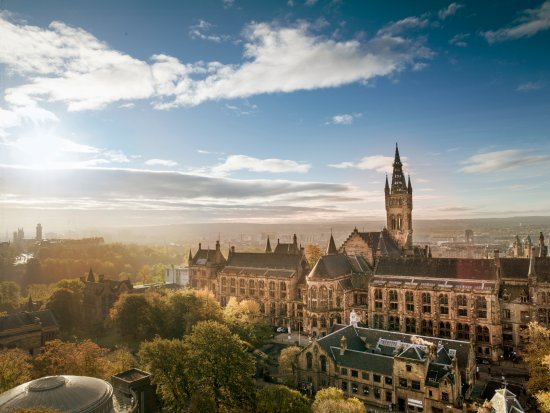
\includegraphics[width=\paperwidth]{background.jpg}}
  \begin{frame}{Thank You!}
    \begin{block}{Dissertation and code available at}
    \url{https://github.com/dilkas/maximum-common-subgraph}
    \end{block}
  \end{frame}
}

\end{document}
